\section{Related Work}
Our method is related to studies on image-to-image translation, sketch-based image generation and face image generation and editing.
In this section, we discuss the most related works of our method. 

\begin{figure}
	\centering
	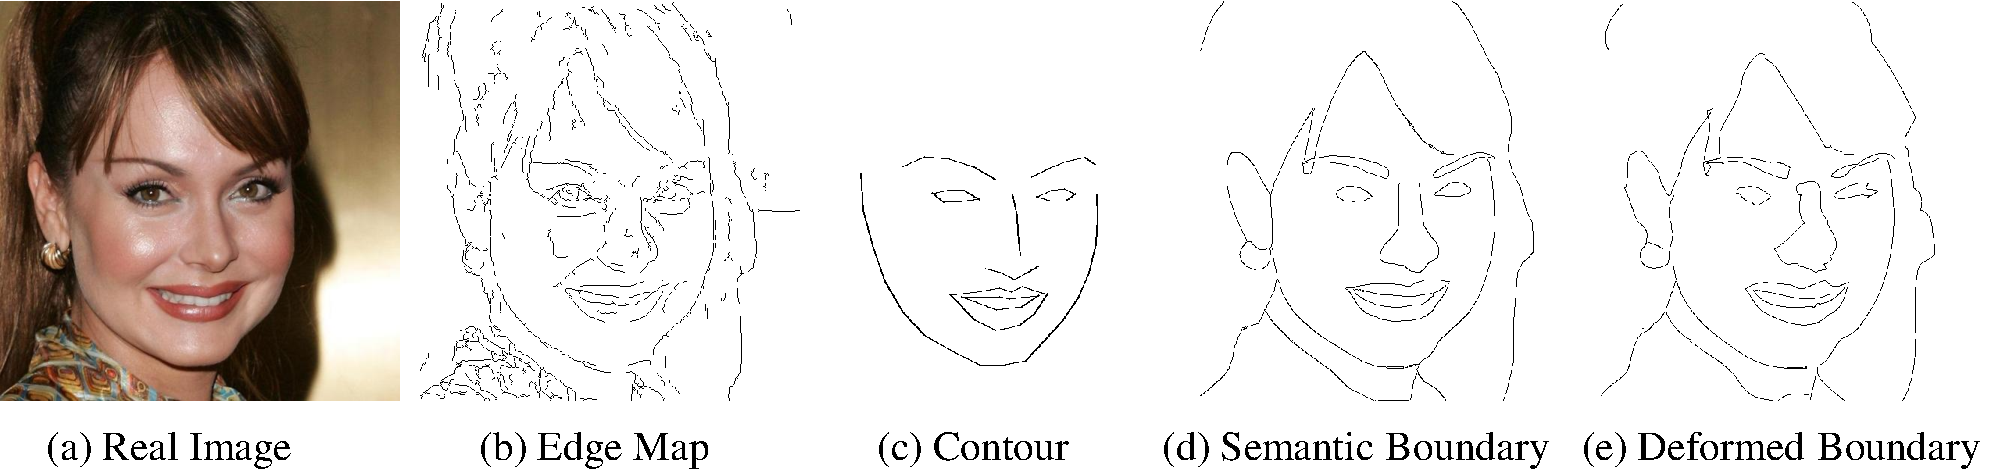
\includegraphics[width=\columnwidth]{figs/data}
	\caption{Comparison between a sketch generated from edge detection and from semantic boundary.}
	\label{fig:sketch_data}
\end{figure}

\subsection{Image-to-Image Translation}
Given an input image from one domain, an image-to-image translation model outputs a corresponding image from another domain and preserves the content in the input image. Existing image-to-image translation models are based on generative adversarial networks conditioned on images. 
%
Pix2pix~\cite{pix2pix} is the first general image-to-image translation model which can be applied to different scenarios according to paired training images, such as, semantic maps to natural images, day images to night images, image colorization, and edge maps to images. 
%
\cite{outdoor_scene} utilizes semantic label maps and attributes of outdoor scenes as input and generates the corresponding photo-realistic images.
%
In order to model multi-modal distribution of output images, BicycleGAN~\cite{BicycleGANs} encourages the connection between the output and the latent code to be invertible.
%
CycleGAN~\cite{CycleGANs}, DualGAN~\cite{DualGANs}, and DiscoGAN~\cite{DiscoGANs} propose unsupervised image translation models with a common idea named cycle consistency, which is borrowed from language translation literature. 
%
Pix2pixHD~\cite{pix2pixHD} is proposed as a high-resolution image-to-image translation model for generating photo-realistic image from semantic label maps using a coarse-to-fine generator and a multi-scale discriminator. It can also be applied to edge-to-photo generation when trained on paired edge maps and photos.
%
However, the large gap between synthesized edge maps and hand-drawn sketches challenges the generalization of these models.

\subsection{Sketch-based Image generation}
Sketch-based image generation is a hot topic in multimedia and computer vision. Given a sketch describe the desired scene layout with text labels for objects, traditional methods, such as Sketch2Photo~\cite{Sketch2Photo} and PhotoSketcher~\cite{PhotoSketcher}, search image patches from a large-scale image dataset and fuse the retrieved image patches together according to the sketch. These methods are not able to ensure the global consistency of the resultant image and fails to generate totally new images.
%
Nevertheless, it is challenging for these methods to ensure global consistency of the resultant images. Thus they frequently fail to generate totally new images.
%
After the breakthrough made by deep neural networks (DNNs) in many image understanding tasks, a variety of DNN-based models have been proposed for sketch-based image generation. 
%
The general image-to-image translation models mentioned above can be easily extended to sketch-based image generation once sketches and their corresponding images are available as training data. 
%
Besides, a few other models are designed specially for sketch inputs. SketchyGAN~\cite{SketchyGAN} aims to generate real images from multi-class sketches. A novel neural network module, called mask residual unit (MRU), is proposed to improve the information flow by injecting the input image at multiple scales. Edge maps are extracted from real images and utilized as training sketches. However, the resultant images of SketchyGAN are still not satisfied.
%
LinesToFacePhoto~\cite{Lines2Face} employs a conditional self-attention module to preserve the completeness of global facial structure in generated face images.
However, this model cannot be generalized to hand-drawn sketches directly due to distinct stroke characteristics.

\subsection{Face Image Generation and Editing}

Recently studies on face image generation and editing have made tremendous progress.
Using generative adversarial network (GAN)~\cite{GANs}, realistic face images can be generated from noise vectors.
%
DCGAN~\cite{DCGANs} introduces a convolutional network \cxj{details} to stabilize training of GAN.
PGGAN\cite{PGGAN} utilizes a progressively growing architecture to generate high resolution face images.
Inspired by style transfer literature, StyleGAN~\cite{StyleGAN} introduces a novel generator which synthesizes plausible high-resolution face images and learns unsupervised separation of high-level attributes and stochastic variation in synthesized images. 
%
On the other side, a number of works focus on face image editing through different control information. StarGAN~\cite{StarGAN-CVPR2018} designs a one-to-many translation framework which switches face attributes assigned by an attribute code. FaceShop~\cite{Faceshop-Portenier-TOG18} and SC-FEGAN~\cite{SC-FEGAN-Jo-ICCV2019} treats sketch-base face image editing as a sketch-guided image inpainting problem where stoke colors is also applied as guidance information. 

